\documentclass[UTF-8,12pt]{ctexart}
\usepackage[english]{babel}
\usepackage{amsmath}
\usepackage{amsfonts,delarray,amsthm,amssymb}
\usepackage{fancyhdr,graphicx,multirow,longtable,booktabs,cite,float,caption}
\usepackage{titlesec,enumerate,xcolor,dsfont,chemarrow,amscd,subfigure}
\usepackage{xeCJK}
\usepackage[margin=1in]{geometry}
\usepackage{url,bm,titletoc,wallpaper}
\usepackage[font=small,labelfont=bf,labelsep=none]{caption}
% ---------------------------------------------------------
\captionsetup{font={footnotesize},labelfont={footnotesize}}
\geometry{left=2.5cm,right=2.5cm,top=2.5cm,bottom=2.5cm}
\CTEXsetup[number={\chinese{section}},format={\Large\bfseries}]{section}
\titleformat{\subsection}{\large\bfseries}{\thesubsection}{1em}{}
\titleformat{\subsubsection}{\large\bfseries}{\thesubsubsection}{1em}{}
%----------------------------------------------------
\def\red{\color{red}}
%------------------------------------------------------
\title{无线能量传输装置}%
\author{洪晟}%

\begin{document}
\makeatletter
\renewcommand{\tablename}{表}
\renewcommand{\figurename}{图}
\renewcommand{\thefigure}{\thesection.\arabic{figure}\quad}
\renewcommand{\thetable}{\thesection.\arabic{table}\quad}
\makeatother

\maketitle
\pagestyle{fancy}
\zihao{-4}

\section{无线能量传输方案设计}



    \subsection{MOSFET器件方案设计}

        {\bf{采用MOSFET器件作为逆变电路的开关管。产生几十Khz的谐振,通过多股并绕的漆包线作为线圈,将能量耦合到次级。}}
        \begin{figure}[H]
          \centering
          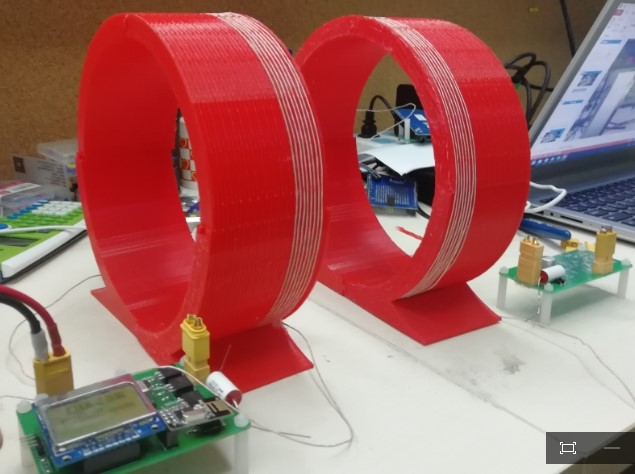
\includegraphics[scale=0.6]{wire1.jpg}
          \caption{MOSFET逆变电路}
          \label{图1 MOSFET逆变电路}
        \end{figure}


    \subsection{GaN器件方案设计}

        {\bf{采用GaN器件作为逆变电路的开关管,产生上兆赫兹的谐振,通过PCB天线作为传输天线,将能量耦合到次级。}}

        \begin{figure}[htbp]
        \centering %居中
        \subfigure[基于GaN器件的全桥功放设计]{                    %第一张子图
        \begin{minipage}{7cm}
        \centering                                                          %子图居中
        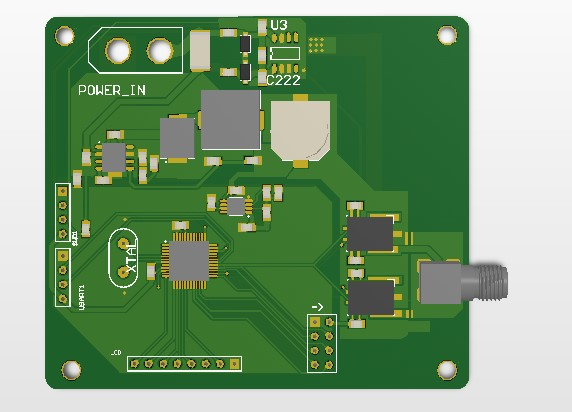
\includegraphics[height=6cm]{GaN1.jpg}               %以pic.jpg的0.5倍大小输出
        \end{minipage}}
        \subfigure[GaN器件PCB天线设计]{                    %第二张子图
        \begin{minipage}{7cm}
        \centering                                                          %子图居中
        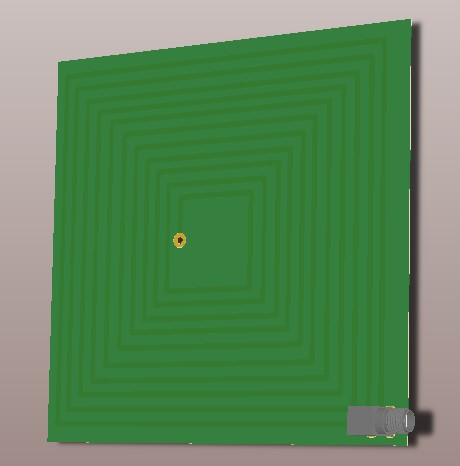
\includegraphics[height=6cm]{GaN1_power.jpg}                %以pic.jpg的0.5倍大小输出
        \end{minipage}}
        \caption{GaN方案设计} %   %大图名称
        \label{GaN方案设计}         % 图片引用标记
        \end{figure}






\section{MOSFET方案设计}

    \subsection{系统硬件框图}

        \begin{figure}[H]
          \centering
          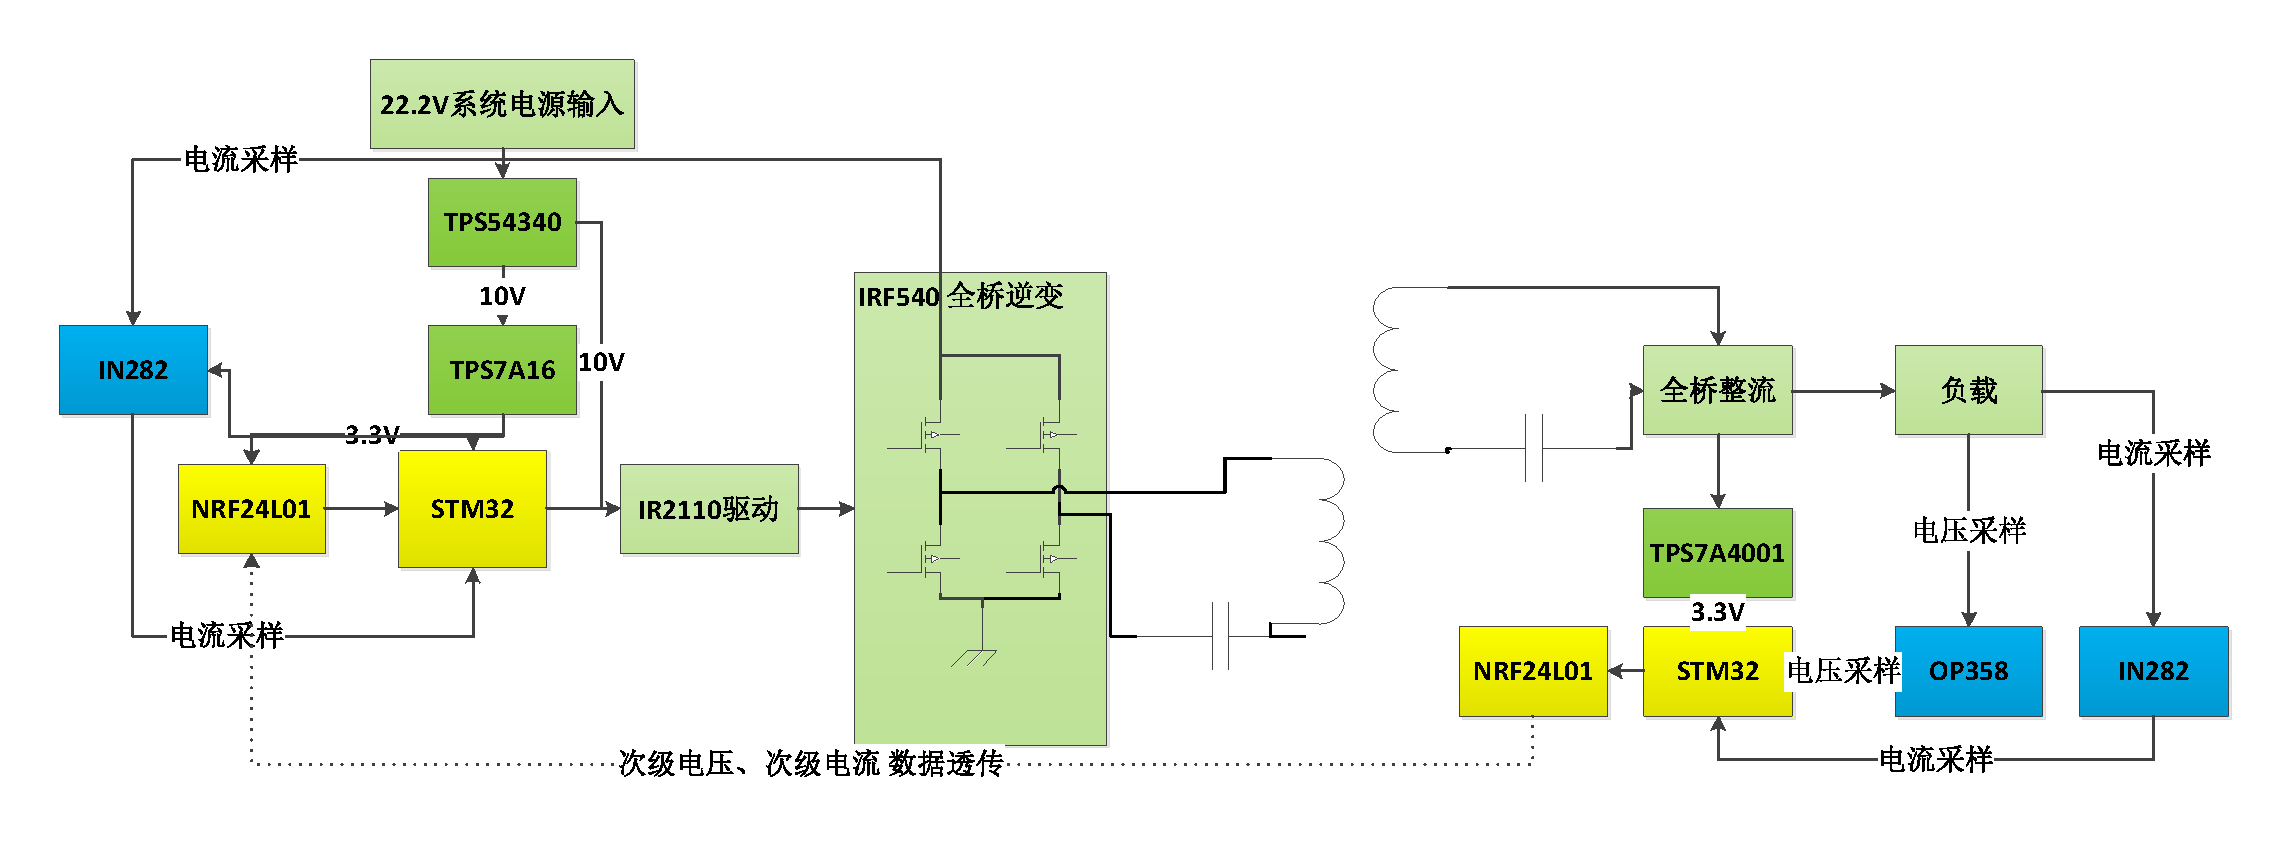
\includegraphics[width=18cm]{sys.pdf}
          \caption{MOSFET方案系统框图}
          \label{sch_MOSFET}
        \end{figure}
        {\bf{
        初级发射原理设计:
        }}
            包含IR2110 2片MOSFET驱动芯片、4个IRF540 MOSFET构成的E类功放谐振电路系统,初级电流采样用于MOSFET过流保护,防止MOSFET 烧坏。NRF24L01 2.4G Zigbee数据透传用于收集次级的电压电流,实现次级的闭环控制。

        {\bf{
        次级接收原理设计:
        }}
            由功率二极管构成的整流电路,包含电流采样、电压采样电路,用于采集负载上的电压电流,并通过NRF24L01透传给初级,作为初级的闭环控制信号。

        \begin{figure}[htbp]
        \centering %居中
        \subfigure[接收端原理图]{                    %第一张子图
        \begin{minipage}{7cm}
        \centering                                                          %子图居中
        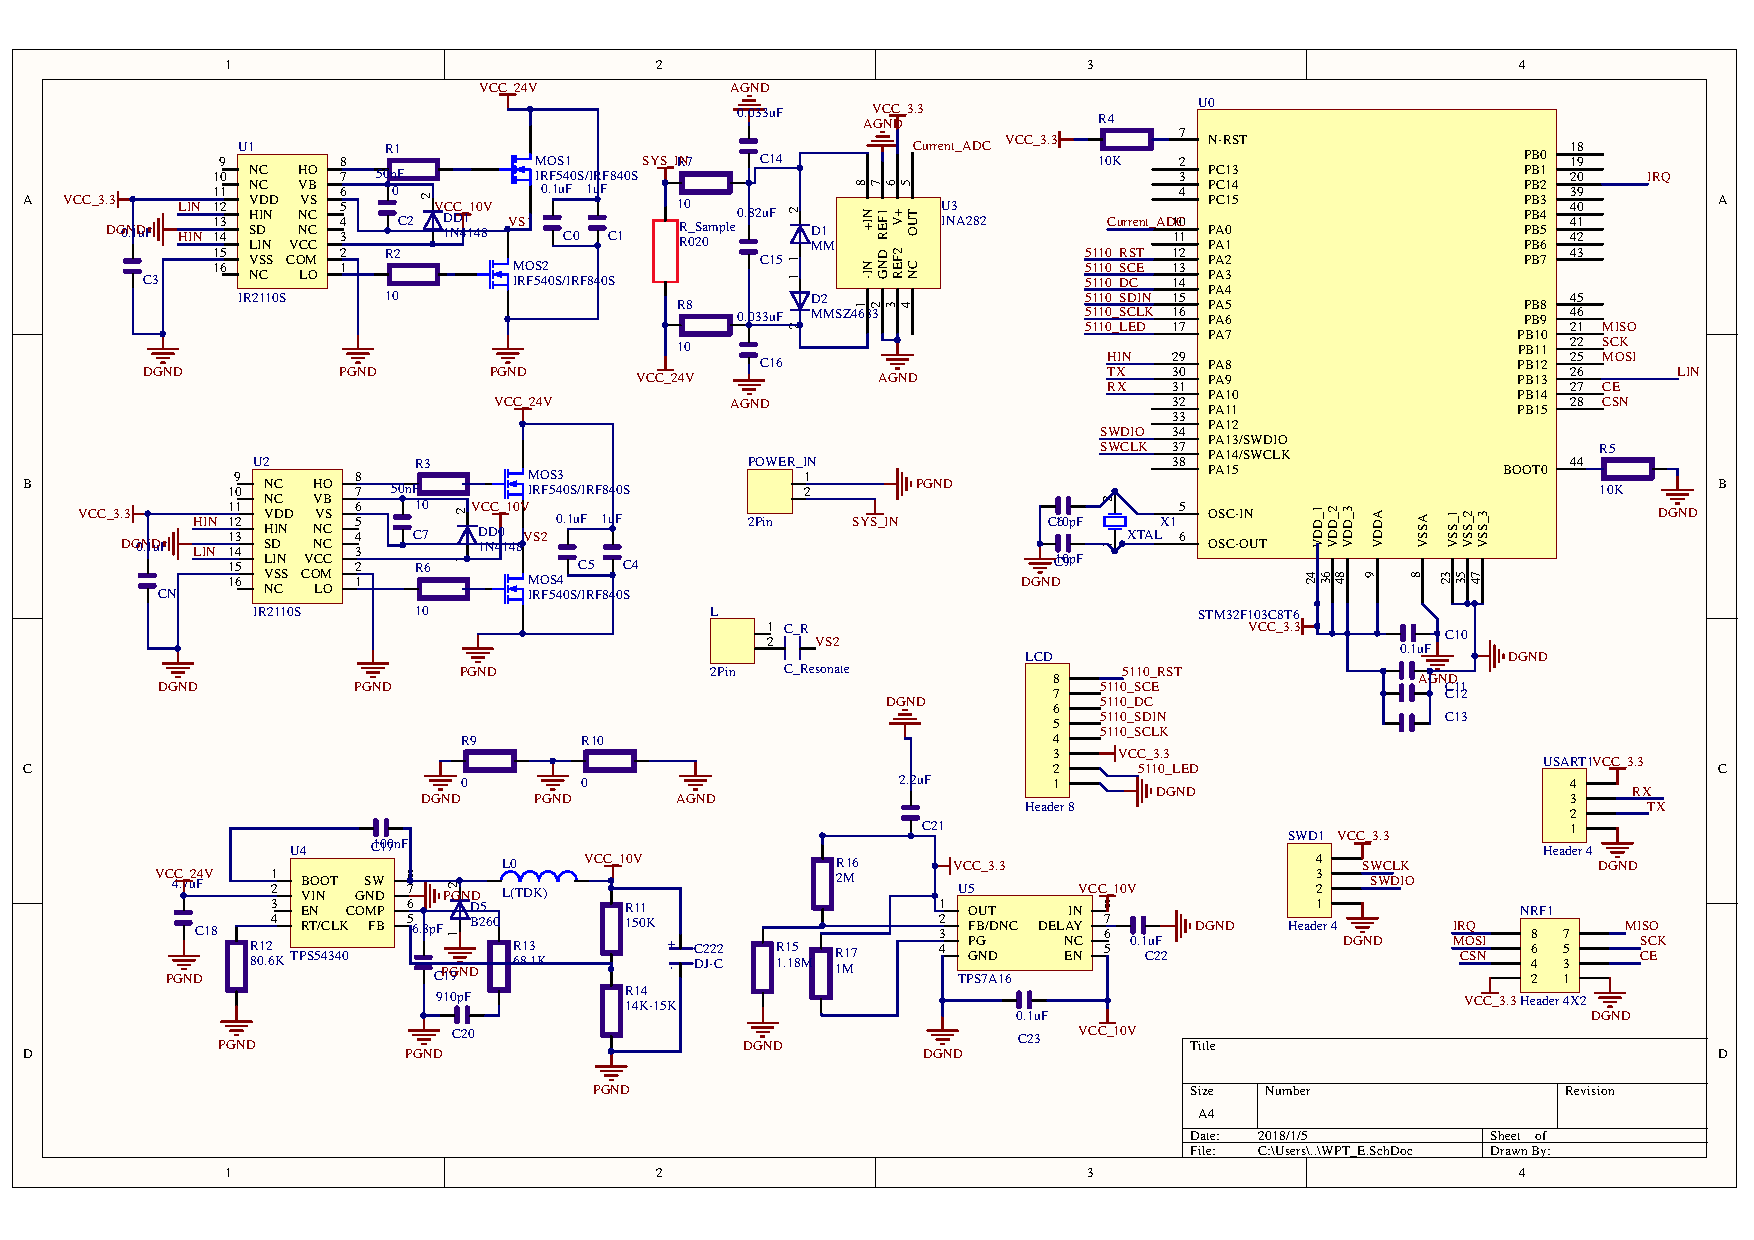
\includegraphics[height=5cm]{WPT_E1.pdf}               %以pic.jpg的0.5倍大小输出
        \end{minipage}}
        \subfigure[发射端原理图]{                    %第二张子图
        \begin{minipage}{7cm}
        \centering                                                          %子图居中
        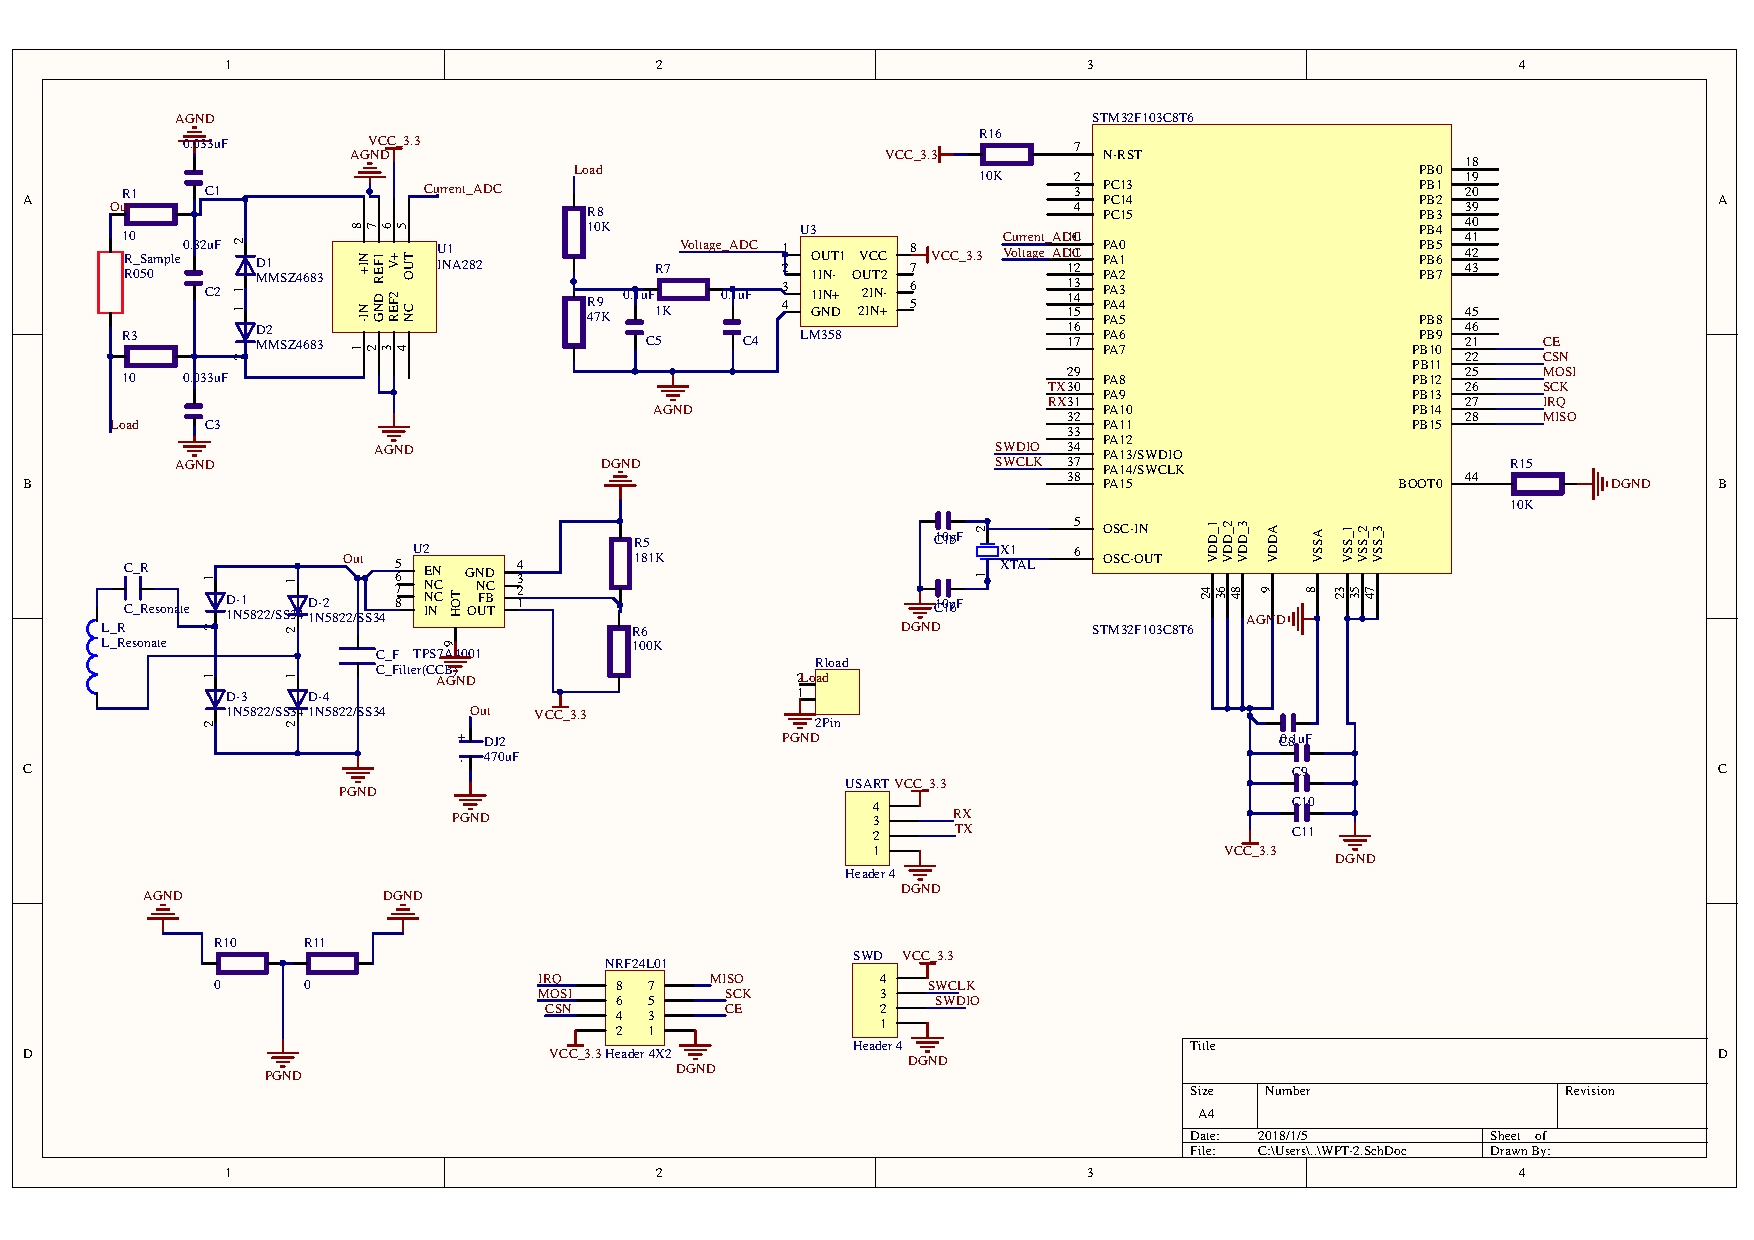
\includegraphics[height=5cm]{WPT-2.pdf}                %以pic.jpg的0.5倍大小输出
        \end{minipage}}
        \caption{MOSFET方案原理图设计} %   %大图名称
        \label{MOSFET方案原理图设计}         % 图片引用标记
        \end{figure}


    \subsection{谐振线圈设计}


            \begin{equation}
            L=N^2\times R \times \mu_0\left[\ln(\frac{8R}{a})-1.75\right]
            \label{L}
            \end{equation}

            式中\[\begin{split}
            &N\text{——线圈匝数} \\
            &\mu_0=4\pi \times 10^{-7}\text{——真空磁导率} \\
            &R\text{——线圈半径} \\
            &a\text{——线圈导线半径} \\
            \end{split}\]

            电感线圈制作,选取{\bf{线径为0.1mm的50股并绕的里兹线制作谐振线圈,铜线的半径为0.05m,另外线圈缠绕8周,线圈半径为0.1m。}}带入估算公式可得出L的数值为: $26.74\mu F$,经过电桥测试,得到实际电感值为:$26.67\mu H$,和估算公式得出的电感值相近。

            电容选用{\red{无极性同轴电容}},ESR较低,品质因数较好。
            经过电桥测试,电容值为:$544.47\mu F$与标定值$550\mu F$相近。

                \begin{figure}[htbp]
                \centering %居中
                \subfigure[电桥测试电感真实值]{                    %第一张子图
                \begin{minipage}{7cm}
                \centering                                                          %子图居中
                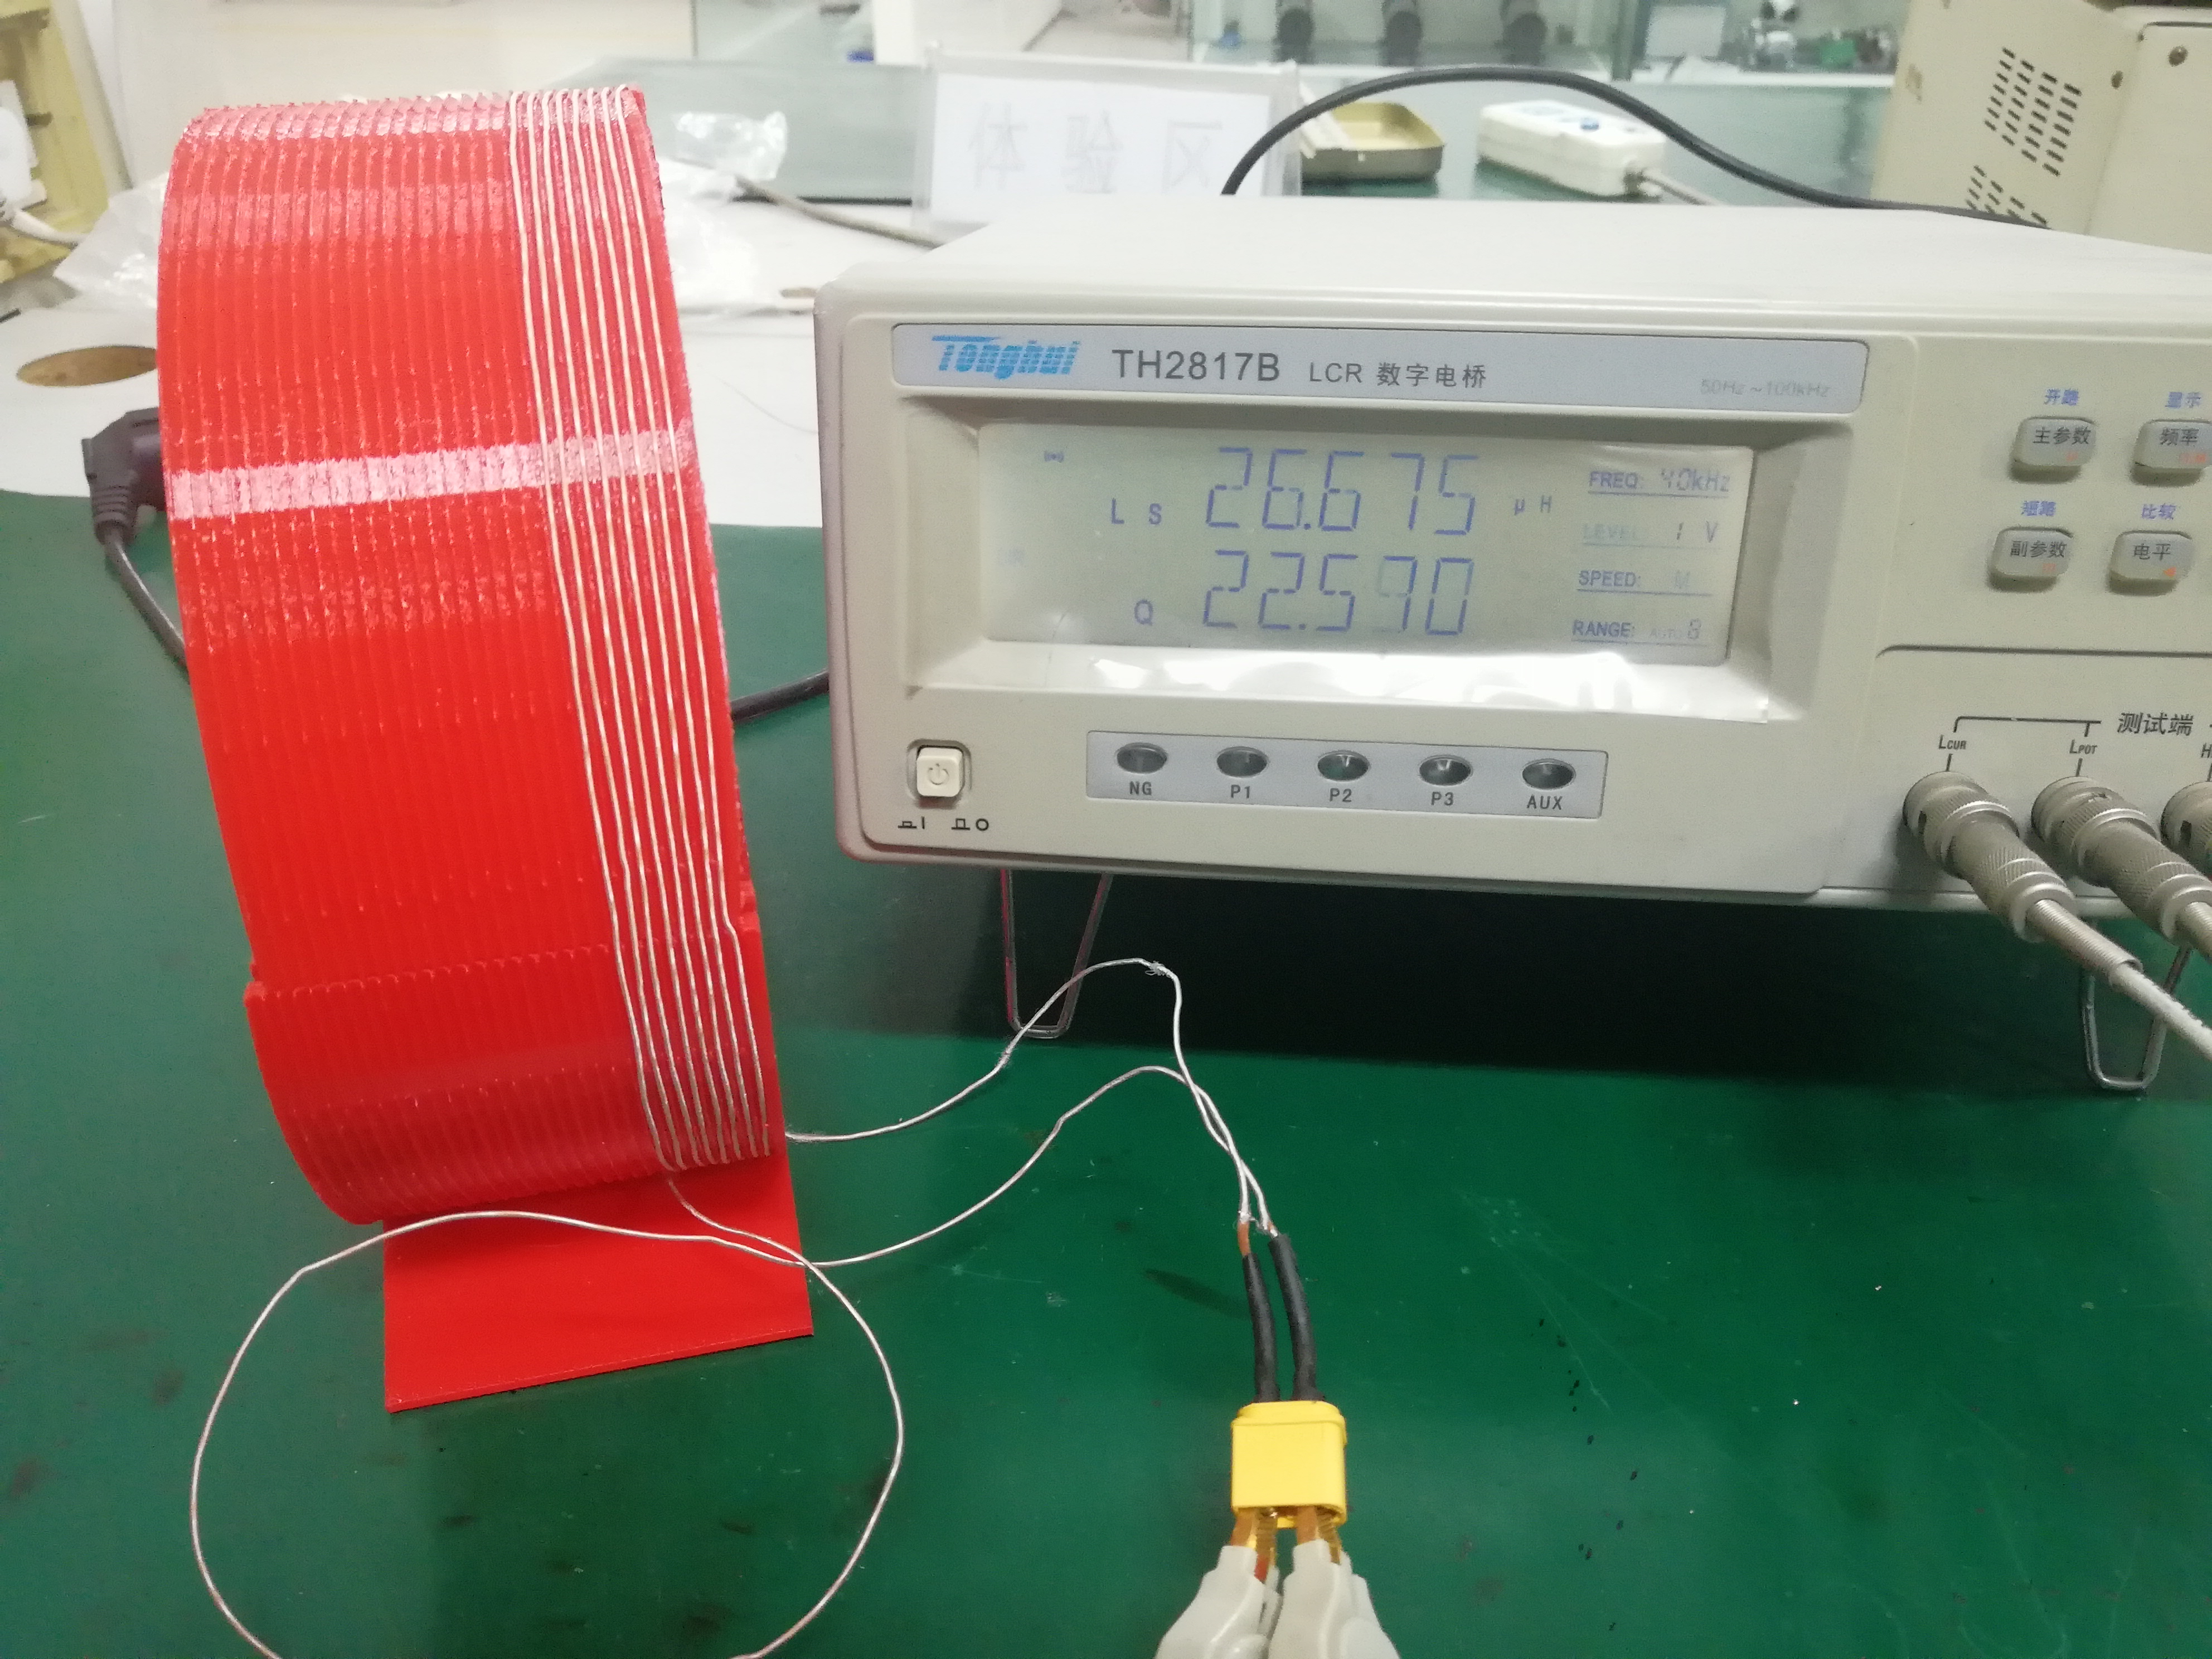
\includegraphics[height=6cm]{e_coil.jpg}               %以pic.jpg的0.5倍大小输出
                \end{minipage}}
                \subfigure[电桥测试电容真实值]{                    %第二张子图
                \begin{minipage}{7cm}
                \centering                                                          %子图居中
                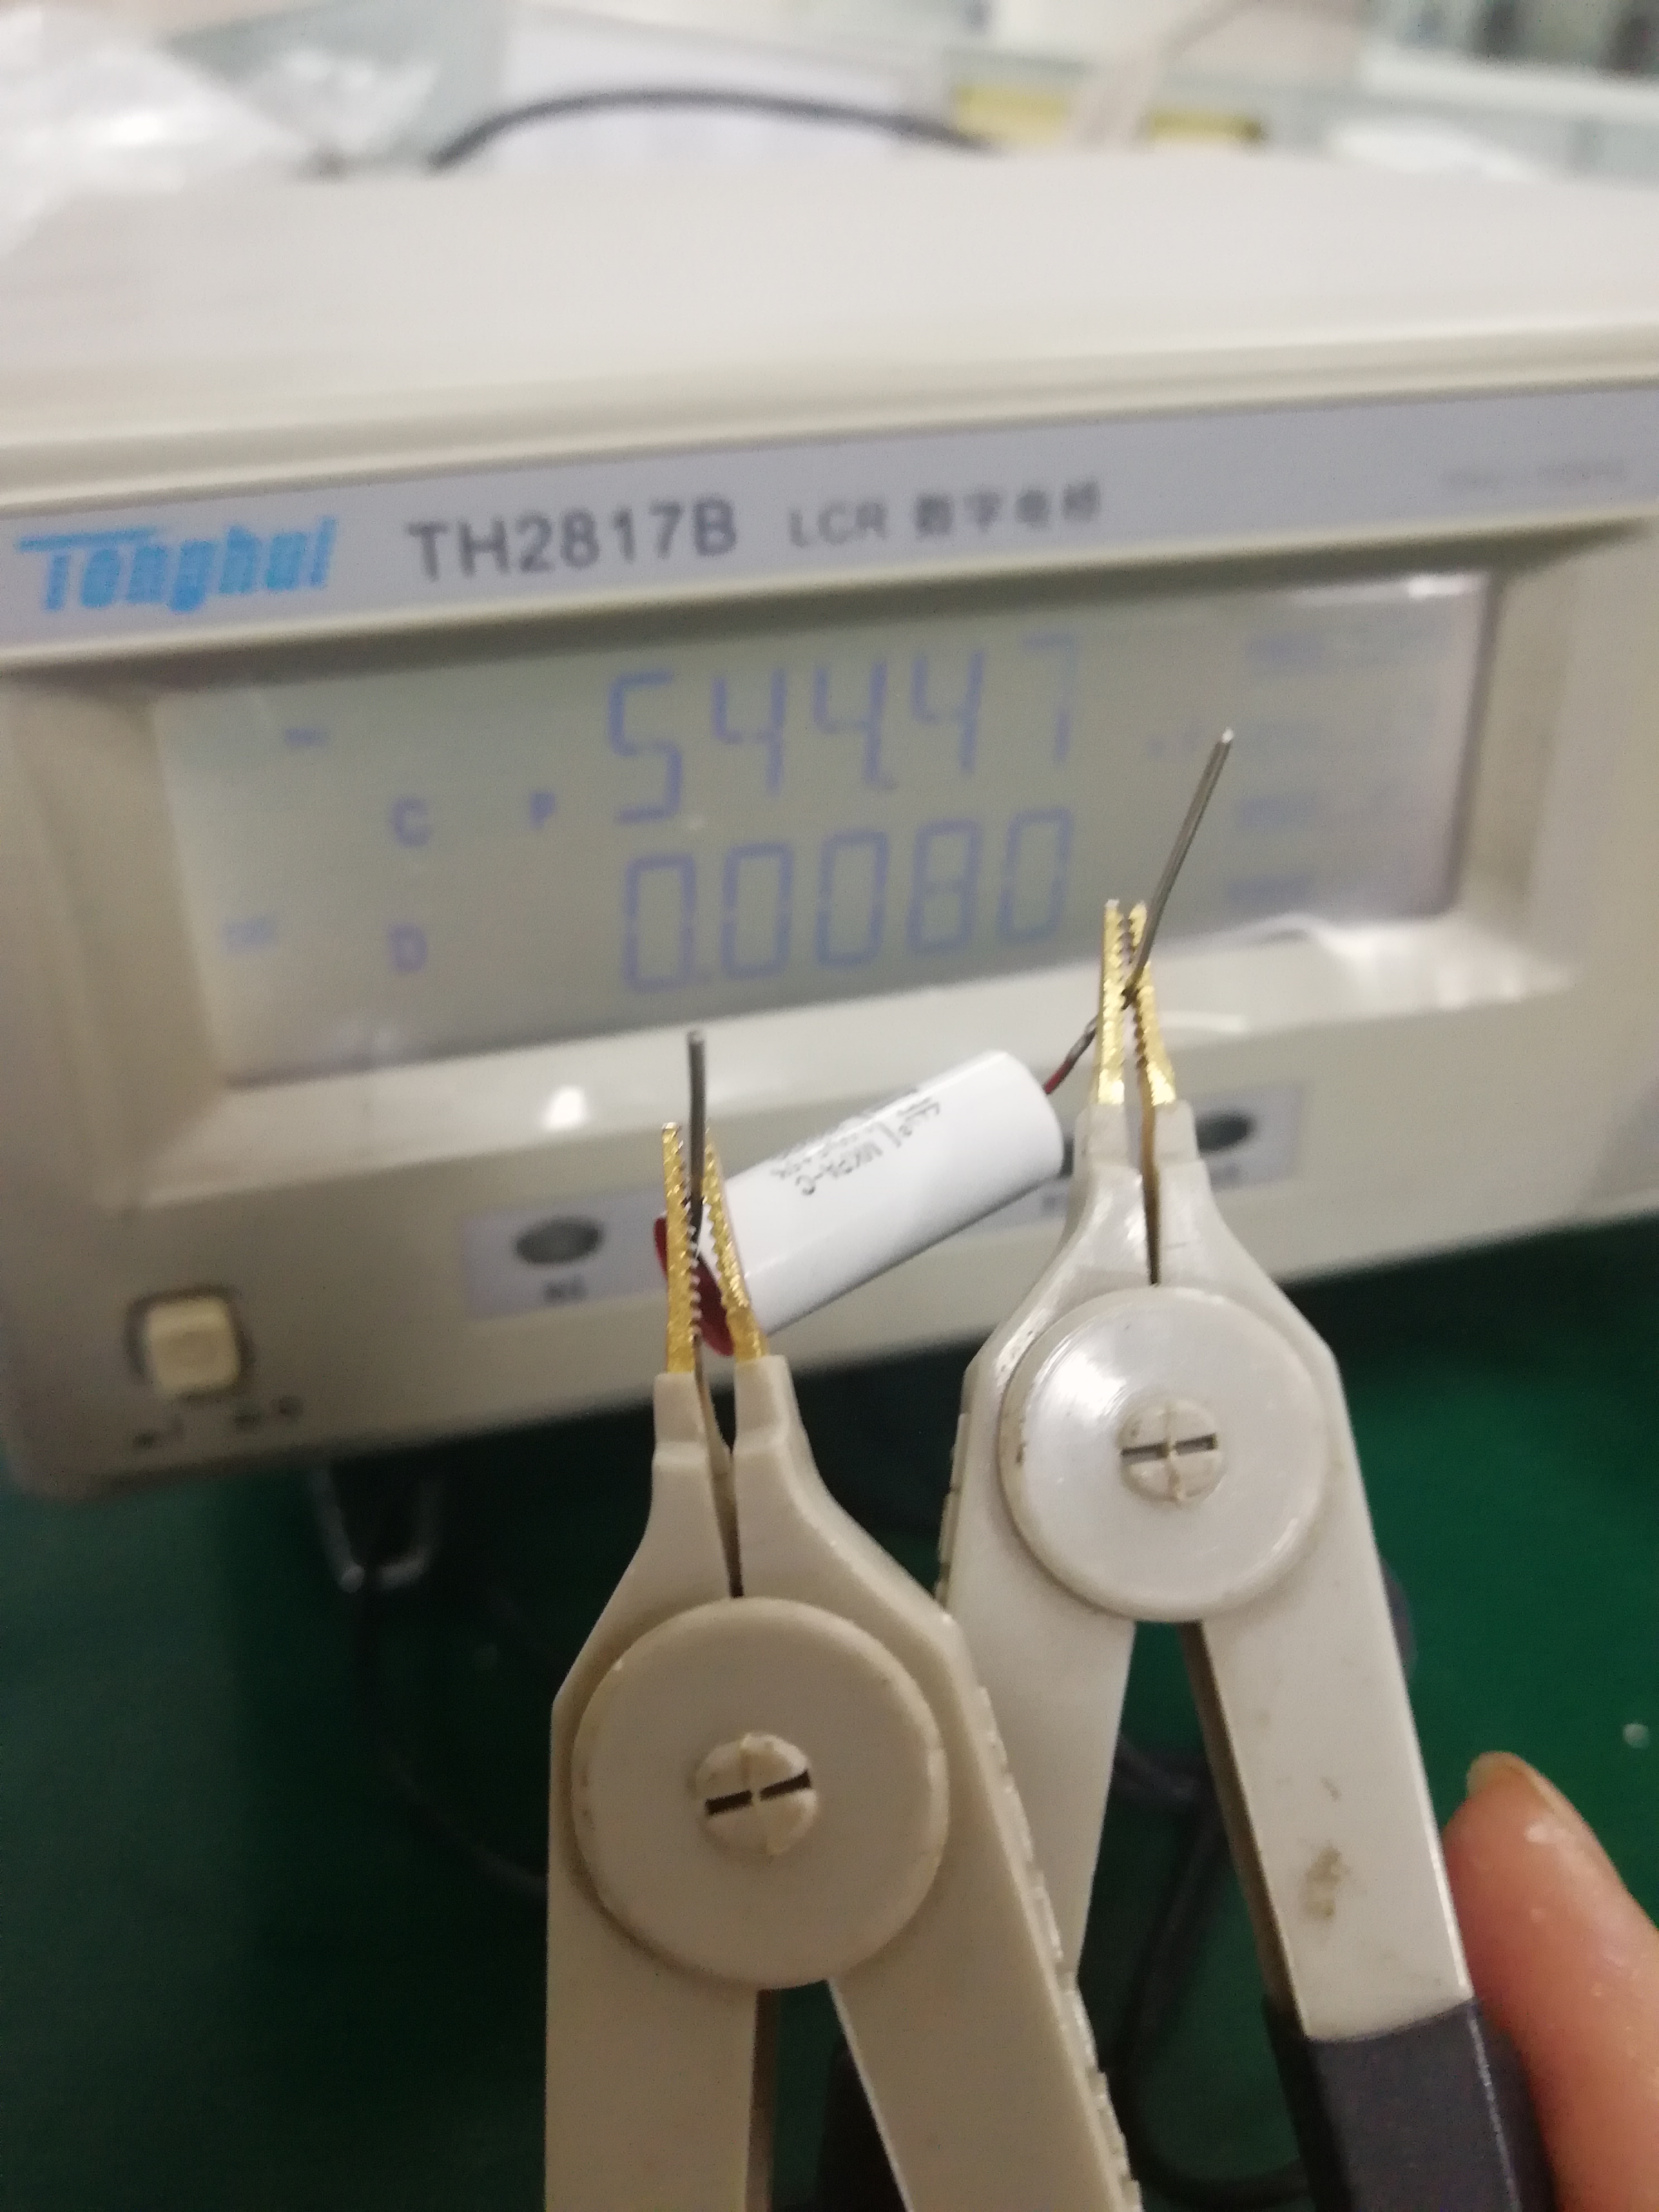
\includegraphics[height=6cm]{CCC.jpg}                %以pic.jpg的0.5倍大小输出
                \end{minipage}}
                \caption{电桥LC参数测试} %   %大图名称
                \label{fig:2}         % 图片引用标记
                \end{figure}

                    \begin{equation}
                    f=\frac{1}{2\pi\sqrt{LC}}
                    \label{frequency}
                    \end{equation}


            将测量得到的L、C的参数带入公式\ref{frequency}可知谐振频率为41.74KHz




    \subsection{程序框图}

            \begin{figure}[H]
              \centering
              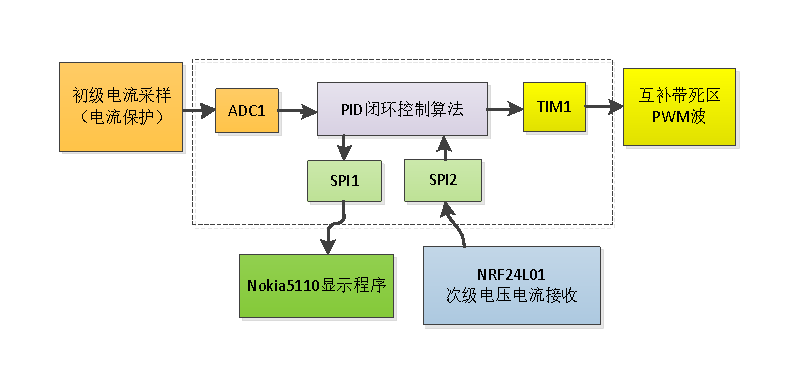
\includegraphics[width=12cm]{pri.pdf}
              \caption{初级发射端程序框图}
              \label{frame_prim}
            \end{figure}
                初级和次级主控制器,采用主频在72Mhz的STM32作为核心处理器,通过TIM1的PWM发生器,参数42Khz的带死区保护的PWM,输出给MOSFET 驱动,在次级感生电压,次级主控板开始工作,并实时回传电压电流信号,初级接收到次级的电压电流信号,执行电压闭环或电流闭环的PID程序。通过SPI接口,读写Nokia5110显示屏,刷新电压电流值。
                另外通过读取ADC1上输入端的电流值,当MOSFET输出电流大于其额定值,PWM的导通时间会减小,用于保护MOSFET 不因长时间大电流烧坏。

            \begin{figure}[H]
              \centering
              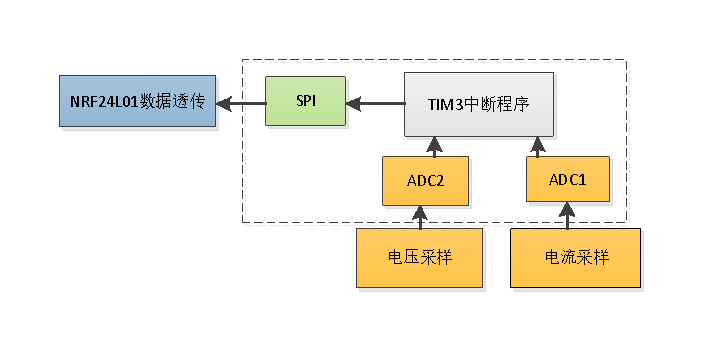
\includegraphics[width=15cm]{sub.pdf}
              \caption{次级接收端程序框图}
              \label{frame_prim}
            \end{figure}
                次级控制器,在定时器TIM3中断程序中读取电压电流的ADC采样数值,并实时通过NRF24L01的Zigbee模块将数据回传给初级。
            \begin{figure}[H]
              \centering
              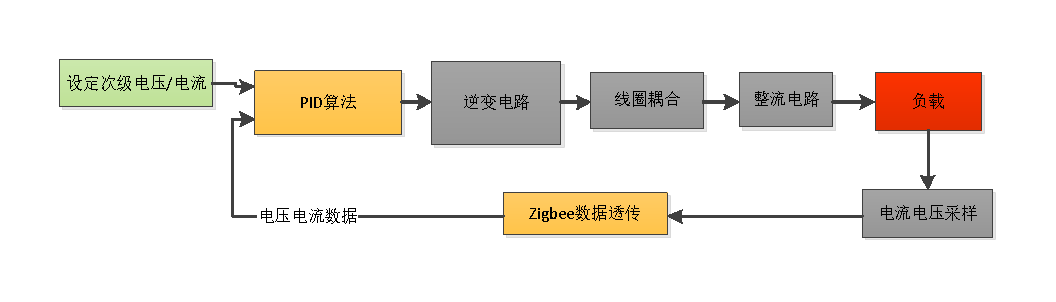
\includegraphics[width=15cm]{control.pdf}
              \caption{PID控制闭环程序框图}
              \label{control}
            \end{figure}


    \subsection{驱动电路}

\section{GaN方案设计}



    \subsection{PCB天线参数验证}
         根据参考文献。设计天线,使用雕刻机雕刻覆铜板,制作PCB天线。
        \begin{figure}[H]
          \centering
          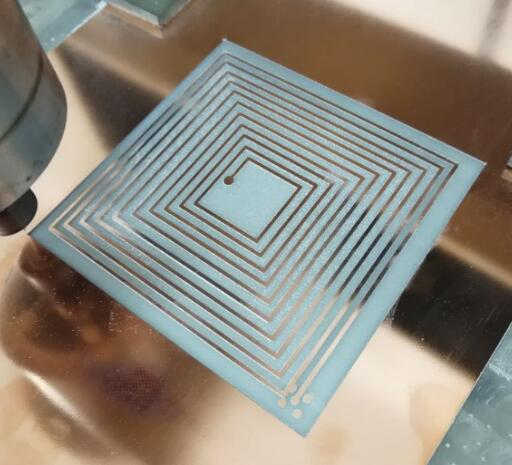
\includegraphics[scale=0.6]{5200.jpg}
          \caption{雕刻的PCB天线}
          \label{幅度变化}
        \end{figure}
        
        \begin{figure}[H]
          \centering
          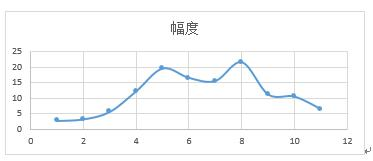
\includegraphics[scale=1]{Amp_power.jpg}
          \caption{扫频时PCB线圈上的幅度变化}
          \label{幅度变化}
        \end{figure}
        {\bf{依据图\ref{幅度变化}可得出线圈的谐振频率在8Mhz时,为最大谐振点。}}





    \subsection{驱动电路}

\section{进度总结}
        \begin{enumerate}[$\bullet$]
        \item 完成MOSFET器件的全桥功放的设计和验证
        \item 使用Solidworks对线圈进行设计,3D打印线圈骨架
        \item 学习HFSS对线圈仿真
        \item 设计了GaN器件的全桥功放
        \item 根据文献参数,制作高频PCB天线
        
        
\end{enumerate}

\[
f=\frac{1}{2\pi\sqrt{LC}}
\]

\[\begin{split}
f &= a+b  \\
  &= c+d  \\
\end{split}\]



% ----end------------------------------------------------------------
\end{document}
% ----------------------------------------------------------------
